\chapter{The ALICE detector at the LHC}
\label{chap:alice}
Founded in 1954, the \gls{cern} research facility in Switzerland was Europe's first scientific joint venture and is now counting 20 member states. \gls{cern} is dedicated to fundamental particle physics research and houses the world's largest particle collider, the \gls{lhc}. 
\section{The Large Hadron Collider}
The \gls{lhc} is a circular particle accelerator situated in the \SI{27}{\km} circumference tunnel of the former \gls{lep} experiment. The operation of the \gls{lhc} requires several pre-accelerators and is depicted in fig.~\ref{fig:lhc_layout}. Initially, protons or Pb ions are accelerated via a linear accelerator and three consecutive synchrotron accelerators. Upon feeding the beam into the final \gls{lhc} ring it is split up into two beams, one circulating through the \gls{lhc} tunnel in a clockwise and the other one in a counter-clockwise direction. The two beams intersect at four specific locations each being the site of one of the four \gls{lhc} experiments: \gls{atlas}, \gls{alice}, \gls{cms} and \gls{lhcb}. Each of these experiments has a specific physical main focus and its own independent collaboration associated to it. The analysis at hand is based on the data collected by the \gls{alice} detector. Hence, only that detector is described in more detail in the following section.
\begin{figure}
  \centering
  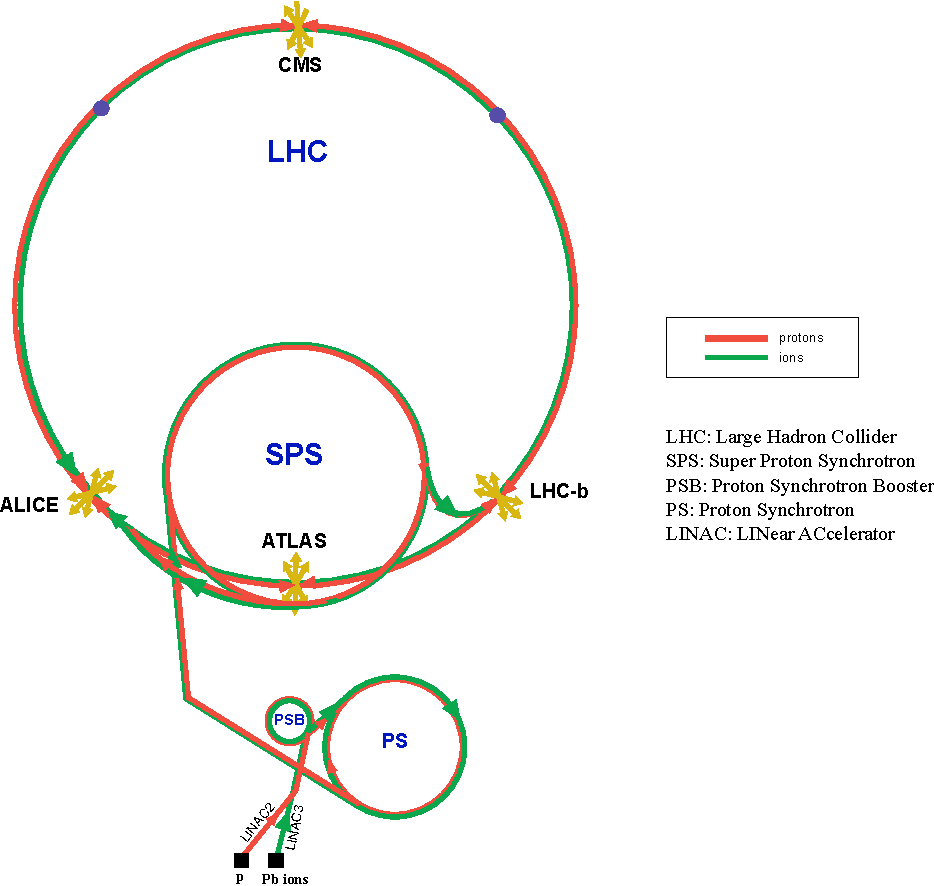
\includegraphics[width=0.8\textwidth]{figures/accelerators_mod}
  \caption[Simplified layout of the LHC, its preaccelerators and the location of the four detector sites.]{Simplified layout of the LHC, its preaccelerators and the location of the four detector sites. With modifications from \cite{Manglunki2001}.}
  \label{fig:lhc_layout}
\end{figure}

\section{ALICE}
\gls{alice} is the single dedicated heavy-ion experiment at the \gls{lhc} and is built by a collaboration of 105 institutes in 30 countries \cite{Collaboration2008}. It focuses on the \gls{qcd} sector of the \gls{sm} described in section \ref{sec:sm}. A detailed description of the \gls{alice} detector can be found in \cite{Collaboration2008} whilst the most important aspects are summarized in this chapter. The detector itself measures $16\times 16\times \SI{26}{m^3}$ and weighs approximately $\SI{10000}{t}$. The center of the experiment is situated \SI{44}{m} under ground. \gls{alice} was planed with \gls{pid} in mind while focusing on the mid rapidity region. Additionally, it was designed in anticipation of the high particle multiplicities expected from previously performed heavy ion experiments and is hence optimized for charged particle multiplicity densities of up to $dN/d\eta = 8000$ but is capable of processing twice that amount.  Furthermore, \gls{alice} possess the means to measure the particles' momenta $p$ from several tens of \si{MeV} up to more than \SI{50}{GeV/c}. The detector also records the specific ionization energy loss $dE/dx$, \gls{tof} information as well as transition and Cherenkov radiation. Together with the employment of electromagnetic calorimetry, muon filters and topological decay reconstruction \gls{alice} includes essentially all known \gls{pid} techniques. The particle tracking capabilities of the detector are outstanding; mainly due to the large volume of nearly $\SI{100}{m^3}$ and the segmentation into $\sim 500,000$ channels that are read out in $1000$ time steps for each event. \gls{alice}'s data acquisition system is capable of writing \SI{1.3}{GB/s} to permanent storage.

\subsection{Detectors of importance to this analysis}
\label{sec:detectors}

\gls{alice} is composed of several individual detector systems and is schematically depicted in fig. \ref{fig:alice_scheme}. The detector consists of a central barrel part (left hand side) and the muon arm (right hand side). The following discusses the components immediately involved in the here presented analysis while reference is again made to \cite{Collaboration2008} for a more complete description. 


\begin{figure}
  \centering
  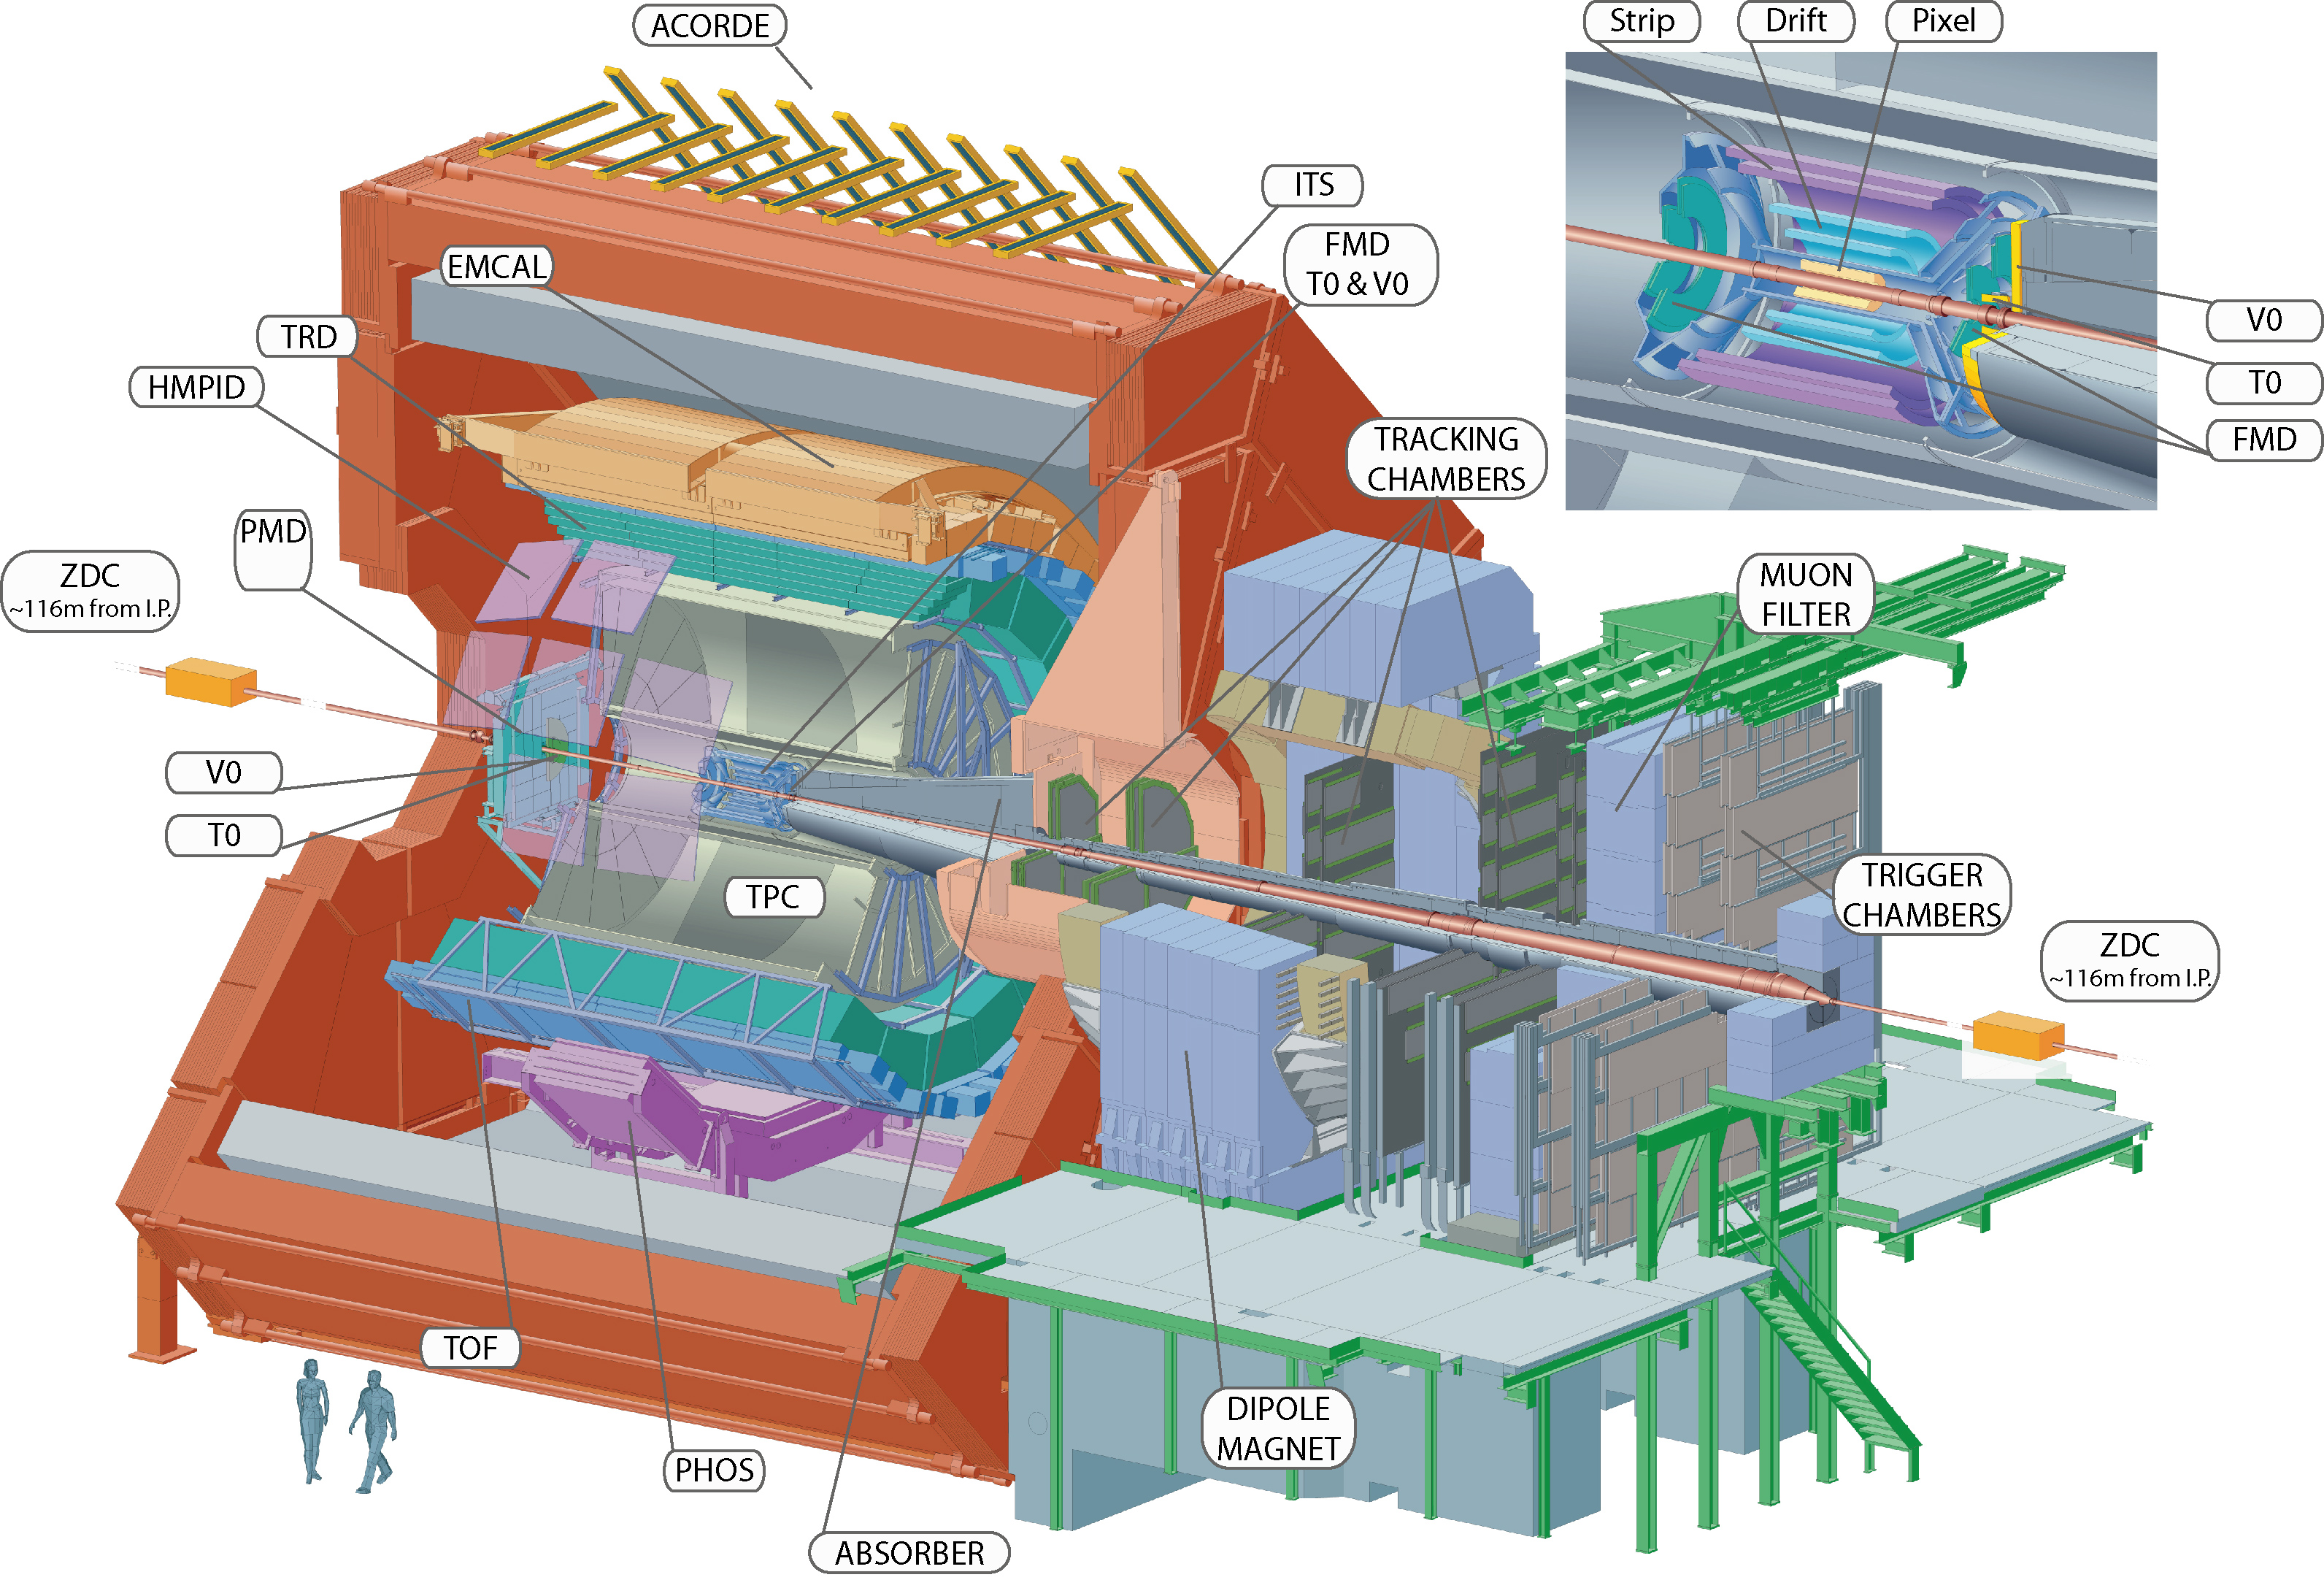
\includegraphics[width=0.9\textwidth]{figures/2012-Aug-02-ALICE_3D_v0_with_Text.jpg}
  \caption[Schematic setup of the ALICE detector.]{Schematic setup of the ALICE detector \cite{alice_3d}}
  \label{fig:alice_scheme}
\end{figure}

\subsubsection{Particle tracking detectors}
\label{sec:tracking_detectors}
Particle tracking is mainly achieved by the \gls{its} and the \gls{tpc}. The former (depicted in the inlay of fig.~\ref{fig:alice_scheme}) is a six layer silicon vertex detector situated immediately around the interaction point, it measures \SI{97.6}{cm} along the beam axis and has a diameter of \SI{87.2}{cm}. The \gls{its} is itself composed of three more detector systems; ordered by increasing distance from the beam pipe they are the \gls{spd}, the \gls{sdd} and the \gls{ssd}. The main purpose of the \gls{its} in this analysis is the localization of the primary vertex with a resolution $\le \SI{100}{\micro \meter}$, an improvement of the momentum and angular resolution of the \gls{tpc} and yielding a criterion for track cut selection (cf. sec. \ref{sec:event_selection}) However, it is also capable of measuring secondary vertices of decaying heavy hadrons and can track particles with a momentum below \SI{200}{MeV/c}. While covering the full azimuthal angle the \gls{its} covers a pseudo rapidity range of $ |\eta |< 1.98$.

The cylindrical \gls{tpc} is the main tracking detector of \gls{alice} and completely encloses the \gls{its}. Its active volume, filled with a mixture of Ne/CO$_2$/N$_2$, reaches from the inner radius of  $\SI{\sim 85}{cm}$ to the outer one of \SI{\sim 250}{cm} and extends parallel to the beam axis for \SI{500}{cm}. Like the \gls{its} the \gls{tpc} covers the full azimuthal angle and a rapidity range of $|\eta | < 0.9$ if the full track length is required. 
The active volume is divided at its center by a aluminized Mylar foil extending perpendicular to the beam axis. In order to achieve a constant voltage gradient towards the ends of the detector of \SI{400}{V/cm} a high voltage of \SI{100}{kV} is applied to the central foil.

An electron created in the active volume by ionization yields a maximum drift time of $\sim \SI{90}{\micro \second}$ until it reaches the end caps of the \gls{tpc} where the readout chambers are situated. Since the track density decreases with increasing radius from the center \gls{alice} has two different readout chambers are segmented radially into an inner and an outer readout chamber. Both of them utilize a \gls{mwpc} to amplify charges drifting towards the read out planes situated immediately underneath.

If a charged particle traverses through the active medium ionization occurs along its trajectory. The created electrons will drift at a constant velocity along the electric field towards the \gls{mwpc} where they cause an avalanche of further electrons inducing a signal in the closest read out pads. This allows the two dimensional projection of the bending track to be measured. By also measuring the precise timing of these signals and knowing the constant drift velocity, it is possible to reconstruct the three dimensional trajectory of all charged  particles traversing the \gls{tpc}.


\subsubsection{Triggering and multiplicity estimation}
The analysis presented here relies on the V0 detector for multiplicity estimation as well as event selection. It consists of two arrays of scintillator counters, V0A and V0C, on opposite sides of the interaction point. The former is situated oppositely from the muon arm and \SI{340}{cm} from the vertex. It covers the rapidity range of $2.8 < \eta < 5.1$. The latter is located \SI{90}{cm} from the vertex while covering the interval of $-3.7 < \eta < -1.7$. The embedding of this detector in the event selection and multiplicity estimation is described in sec.~\ref{sec:event_track_selection}.

%%% Local Variables: 
%%% mode: latex
%%% TeX-master: "main"
%%% End: 
